\subsection{\RU{Чтение за пределами массива}\EN{Reading outside array bounds}}

\RU{Итак, индексация массива\EMDASH{}это просто \IT{массив\lbrack{}индекс\rbrack}.  % TODO1 как-то плохо отображаются []
Если вы присмотритесь к коду, в цикле печати значений массива через \printf вы 
не увидите проверок индекса, \IT{меньше ли он двадцати?} 
А что будет если он будет 20 или больше? 
Эта одна из особенностей \CCpp, за которую их, собственно, и ругают.}
\EN{So, array indexing is just \IT{array\lbrack{}index\rbrack}.
If you study the generated code closely, you'll probably note the missing index bounds checking,
which could check \IT{if it is less than 20}.
What if the index is 20 or greater?
That's the one \CCpp feature it is often blamed for.}

\RU{Вот код, который и компилируется и работает:}
\EN{Here is a code that successfully compiles and works:}

\lstinputlisting{patterns/13_arrays/2_BO/r.c}

\RU{Вот результат компиляции в}\EN{Compilation results} (MSVC 2008):

\lstinputlisting[caption=\NonOptimizing MSVC 2008]{patterns/13_arrays/2_BO/r_msvc.asm}

\RU{У меня данный код при запуске выдал вот такой результат:}\EN{When I run it, I get:}

\begin{figure}[h]
\centering
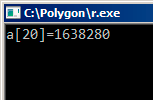
\includegraphics[scale=\NormalScale]{patterns/13_arrays/2_BO/olly_r3.png}
\caption{\olly: \RU{вывод в консоль}\EN{console output}}
\label{fig:array_BO_olly_r3}
\end{figure}

\RU{Это просто \IT{что-то}, что волею случая лежало в стеке рядом с массивом, 
через 80 байт от его первого элемента.}
\EN{It is just \IT{something} that was lying in the stack near to the array, 80 bytes away from its first element.}

\ifdefined\IncludeOlly
\clearpage
\index{\olly}
\RU{Попробуем узнать в \olly, что это за значение}\EN{Let's try to find out where did this value
come from, using \olly}.
\RU{Загружаем и находим это значение, находящееся точно после последнего элемента массива:}
\EN{Let's load and find the value located right after the last array element:}

\begin{figure}[H]
\centering
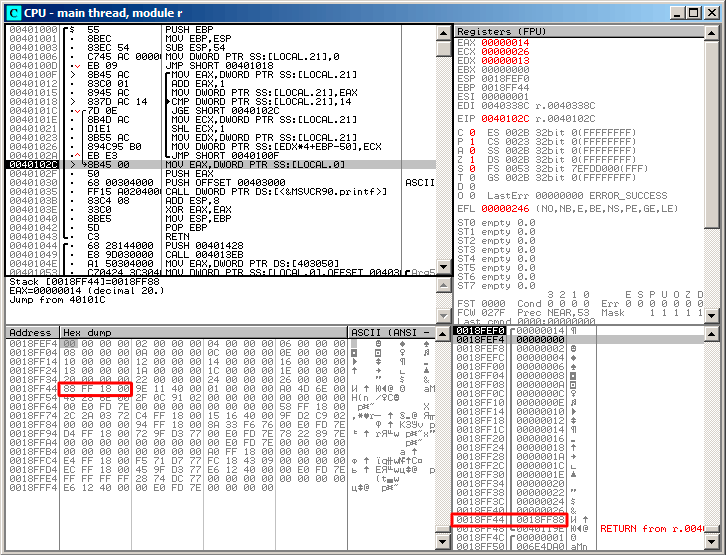
\includegraphics[scale=\FigScale]{patterns/13_arrays/2_BO/olly_r1.png}
\caption{\olly: \RU{чтение 20-го элемента и вызов \printf}\EN{reading of the 20th element and execution of \printf}}
\label{fig:array_BO_olly_r1}
\end{figure}

\RU{Что это за значение}\EN{What is this}? 
\RU{Судя по разметке стека, это сохраненное значение регистра EBP}\EN{Judging by the stack layout,
this is the saved value of the EBP register}.
\clearpage
\RU{Трассируем далее, и видим, как оно восстанавливается}\EN{Let's trace further and see how
it gets restored}:

\begin{figure}[H]
\centering
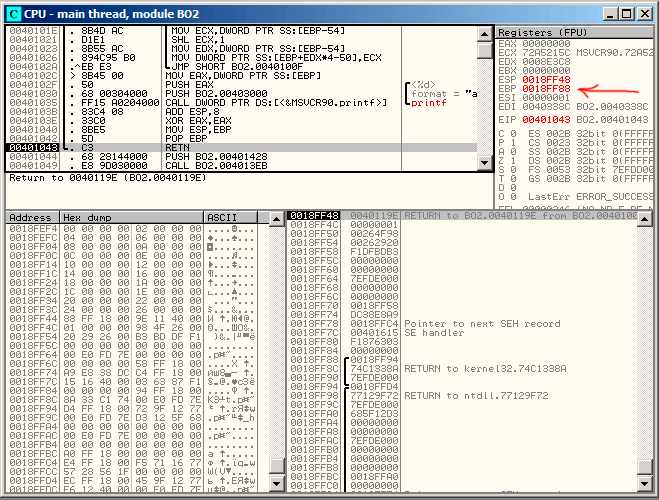
\includegraphics[scale=\FigScale]{patterns/13_arrays/2_BO/olly_r2.png}
\caption{\olly: \RU{восстановление EBP}\EN{restoring value of EBP}}
\label{fig:array_BO_olly_r2}
\end{figure}

\RU{Действительно, а как могло бы быть иначе? Компилятор мог бы встроить какой-то код, 
каждый раз проверяющий индекс на соответствие пределам массива, как в языках программирования 
более высокого уровня\footnote{Java, Python, \etc{}.}, что делало бы запускаемый код медленнее.}
\EN{Indeed, how it could be different?
The compiler may generate some additional code to check the index value to be always
in the array's bounds (like in higher-level programming languages\footnote{Java, Python, \etc{}})
but this makes the code slower.}

\fi
